\documentclass[index]{subfiles}

\begin{document}
\title{Investigating the efficiency of Cheney stop-and-copy and LISP 2 style mark-compact garbage collection algorithms}
\date{}
\author{}
\maketitle

\section{Research Question}

How does the runtime and collection performance of Cheney's stop-and-copy algorithm compare to the LISP 2 mark-compact algorithm?

\section{Introduction}

Garbage collectors, and the algorithms they use, are incredibly widespread in just about any application one can find in the modern day.

One example of these are higher-level programming languages. Javascript is the sole programming language of the web, and drives the functionality of all webpages. Python is the most popular and rising programming language of today and drives artificial intelligence development. Java, a still very popular programming language encodes Minecraft, one of the most popular games of the world, played by millions, and is used in tons of server-side applications worldwide.

The element that these programming languages all have in common is that they are interpreted languages, and they automatically manage memory, by using garbage collectors.

It thus follows that the algorithms behind garbage collection and their relative efficiencies are ever more important to consider, now that more interpreted languages are being run on more and more devices over time. One recent study on this subject has explored the performance differences between different languages running the same program \cite{programming_languages_electricity}, comparing interpreted languages such as Java and Python with manually managed languages such as C++ and Rust. However, the results didn't specifically test garbage collection algorithms specifically, and as each language implements and makes its own tweaks to its own unique garbage collection algorithm, it's hard to say if one base garbage collection algorithm is better than the other using these results alone.

Other contemporary research on the subject has become increasingly complex, factoring in new algorithms or combining old algorithms, however, many assume the basic algorithms as known information, and haven't tested simple algorithms on modern hardware. This paper aims to shed light on the essential component of higher level languages that many programmers tend to look over, presenting information in an easily digestible way, as well as applying that knowledge practically by implementing a simple stop-and-copy and mark-compact garbage collection algorithm in the same programming language in an abstracted way, and comparing the performance of the two in this controlled environment.

\subsection{Methodology}

To fully compare and contrast the differences between these two algorithms, as well as to make educated analysis of the results later, a basic understanding of how memory works in a program, the basic terminology concerning memory management, and what garbage is needs to be researched and understood.

Then research will be done on the basic steps in each algorithm: including when garbage collection is run, how live objects are determined, and what objects are moved where during the compaction process of each algorithm. This will be accompanied by code snippets of how the algorithms are implemented in this paper in the Rust programming language.

Next, the collection performance of each algorithm (how long it takes to clean up the garbage) as well as the runtime performance of each algorithm, (such as accessing the data structure and its values during a traversal of the memory) will be tested and the results recorded.

Finally, research will be done on the basics of hardware caches and organization of memory in modern systems, as one algorithm or another due to its compaction process could support a faster runtime of the program after collection of garbage, and this information will be used to critically analyze the results of the performance of the two algorithms.

\section{Background}

\subsection{The concepts of memory management (explained in the context of a game)}

\begin{quote}
    Imagine a game with multiple enemies. How does one store, add, and remove an enemy?
\end{quote}

The above question basically defines memory managment.

One might first believe that a plain vector might take care of managing the enemies.

\begin{minted}[breaklines]{rust}
    enemies = [enemy1, enemy2, enemy3]
\end{minted}

Whenever one wants to spawn an enemy, it is \textit{allocated} to the vector

\begin{minted}[breaklines]{rust}
    enemies.push(enemy4)
    // enemies = [enemy1, enemy2, enemy3, enemy4]
\end{minted}

And whenever one wants to despawn an enemy, one deallocates it from the vector

\begin{minted}[breaklines]{rust}
    enemies.remove(0)
    // enemies = [enemy2, enemy3, enemy4]
\end{minted}

However, the size of physical memory, one a garbage collector has to deal with, unlike a vector, cannot be freely removed or changed.

Imagine that the vector storing the enemies must be of a fixed length, and one couldn't push or pop from the array at will. Now how would one manage ``alive'' and ``dread'' enemies?

In this array, one would have to keep track of where the next free space is, in order to write to that free space when an enemy should be allocated.

\begin{minted}[breaklines]{rust}
    // enemies = [enemy1, enemy2, enemy3, NULL]
    free = 3
\end{minted}

This simple action of keeping track of the free space, is where all the problems of memory management comes from.

\subsection{In the context of computers}

The data of all computer programs are stored in a place we call memory.

Whenever one wants to make room for new data, one must allocate memory to free space. And whenever one wants to remove data, one must deallocate that memory, back into free space.

In modern computers, there are two places where the program can allocate memory: the stack and the heap.

In the stack, whenever one wishes to allocate something, all one has to do is bump a pointer's memory address up to determine where our next boundary of free memory is \cite{the_rust_programming_language}. However, whenever one wishes to deallocate memory, they must do so from top to the bottom.

Thus, the stack always consists of a block of contiguous used memory, and a block of contiguous free memory.

\begin{minted}[breaklines]{rust}
    free = 4
    memory = [data1, data2, data3, NULL, NULL, NULL]
\end{minted}

However, most of the memory of programs aren't allocated linearly and deallocated in the exact opposite order.

Thus, garbage collection is most concerned with the heap, which, on the other hand, can be accessed at random, and objects with dynamic sizes (that is, that is, sizes unknown at the time we compile our program) can be allocated on the heap. Deallocation of the heap may occur in a random order.

However, the question then becomes, how do we keep track of which sections of the heap are ``free'' memory, and which sections are ``used'' memory on the heap? That's the essence of memory managment.

\subsection{Memory Management Techniques}

There are several ways to manage memory in a language. One is by manually allocating and deallocating: the programmer specifies exactly how much memory is needed at a specific time, and decides when something should be deallocated. In lower-level languages, this is normal. However, manual allocation often requires a lot of experience to learn, and even with it, requires much more time to think about and write a program. It could also easily result in many types of bugs, such as using memory that is already freed, freeing memory twice, and not freeing memory in the first place \cites{garbage_collection_overview_uw}[Chapter~1]{gc_handbook}

Hence, to alleviate the burden of having to keep track of manual memory management, many modern programming languages use automatic memory management. There are many different ways to automatically manage memory. The only types of garbage collectors this paper is concerned with are tracing garbage collectors, which, as their name suggests, directly check objects to determine if they are ``alive'' (used by the program) or ``dead'' (not in use any longer) \cite{a_unified_theory_of_garbage_collection}. In other words, tracing garbage collectors specifically determine if an object is accessible (garbage) or not by traversing some kind of tree \cite[Chapter~1]{gc_handbook}.

The main concept of garbage collection is simple: whenever we want to create a new object, we call \verb+allocate()+, and calculate the new free space on the heap. But if the heap is full, or if we wish to collect the garbage at any time, then we call \verb+collect()+ \cite{gc_handbook}, which as the name suggests, makes the bulk of the garbage collector.

\subsection{LISP-2 Sliding Mark-Compact Algorithm}

One easy to implement type of mark-compact garbage collector is the \textit{sliding} LISP 2 mark-compact garbage collection algorithm.

\begin{figure}[H]
    \centering
    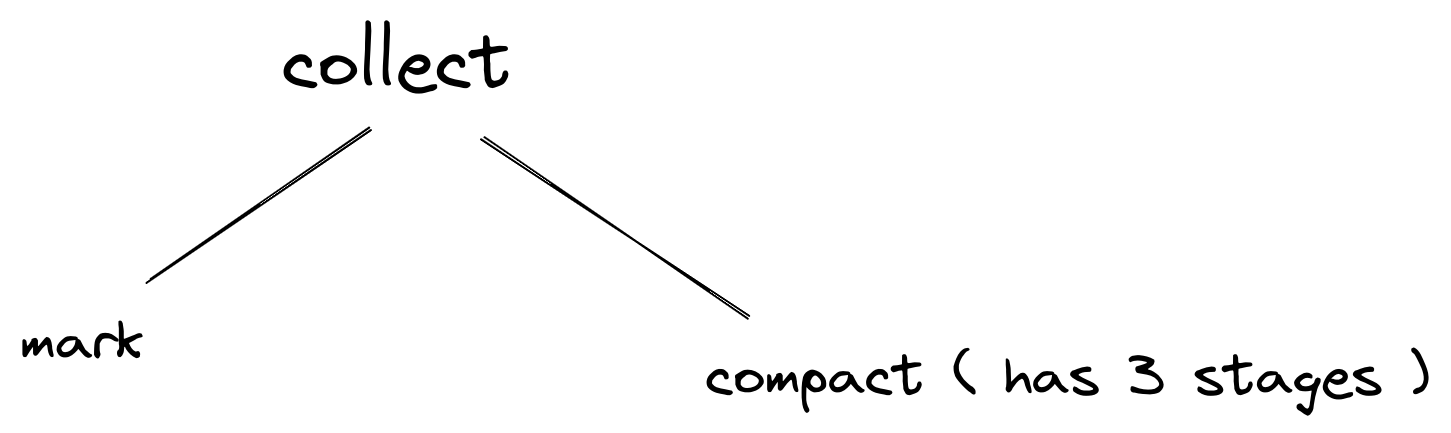
\includegraphics[scale=0.3]{pics/mark-compact-overview.png}
    \caption{Basic overview of mark-compact algorithm}
\end{figure}

The \verb+collect()+ function of this mark-compact algorithm can be broken down into two stages: the \verb+mark()+ stage, where we find out which objects are ``living'' and the \verb+compact()+ stage, where we perform a series of computations to ``slide'' the living objects down into one end, compacting the heap in the process and freeing up space \cite[Chapter~3]{gc_handbook}.

\subsubsection{The Marking Stage}

To determine which objects are alive and dead, we attempt to traverse the entire heap through the graph of objects. We start from the root nodes, located on the stack\cites[3..~Marking]{redhat_openjdk}[Chapter~3]{gc_handbook}, adding the objects that they reference to a worklist. Then we do the same for the worklist. Accessible objects are objects that can eventually be reached by this recursion of reference from the roots. We could use either breadth-first, or depth-first traversal to traverse the heap depending on the implementation (our program uses breadth-first), and objects that are then found to be inaccessible (because they are unmarked) are defined as `garbage' and can be ignored in the \verb+compact+ phase.

\begin{minted}[linenos, breaklines]{rust}
// this block contains the code to mark all reachable objects
{
    // first create a worklist, which is going to be a queue, since
    // we're doing breadth-first traversal
    let mut worklist: VecDeque<NodePointer> = VecDeque::new();

    // populate the worklist with children reachable from the roots
    for root in &stack.roots {
        for child in &root.children {
            worklist.push_back(*child);
        }
    }

    // then we just keep on taking from the worklist until it's empty
    while let Some(node) = worklist.pop_front() {
        // if the node isn't marked (already)
        if !self.is_marked(node) {
            // we mark it because it means it's accessible
            self.mark(node);
            // then add the rest of its children to the back of the queue
            for child_node_pointer in &self.get(node).unwrap().children {
                worklist.push_back(*child_node_pointer);
            }
        }
    }
}
// now all our reachable objects should be marked, everything that isn't is
// considered garbo. We only care about the marked objects in our traversals
// from now on
\end{minted}

As seen by the implementation above, in order to ``mark'' an object that is accessible, the field used to store the forwarding address used for later calcualtions is mutated, which effectively functions as a mark bit to flag that the object. \cite[Chapter~1]{gc_handbook}

% As for storing whether an object is marked with a starting bit, a rather expensive but easy to implement option is to use a bitmap (an array of bits, basically) where each index corresponds to each object in the heap, which is marked 1 or 0 to show that it is alive (1) or dead (0) \cite[Chapter~3]{gc_handbook}.

\subsubsection{Compact Stage}

The compaction stage of the mark-compact algorithm can be broken down into three parts, and in each part, the heap is traversed in its entirety. The first stage is to calculate the location of where the living object will slide down after copying. We do this by initializing a \verb+free+ pointer starting at the very bottom of the heap, and set the \verb+forwarding_address+ of the living marked object in question to the free pointer, then bumping its size up \cites[Chapter~3]{gc_handbook}[Sections~3.3-3.5]{redhat_openjdk}.

\begin{minted}[linenos, breaklines]{rust}
// the next three blocks contain the compact code
// free starts at 0, the beginning of the point which we wish to compact to
let mut free = 0;

// 1. the first step is to calculate new locations of all objects
{
    // we iterate over all objects in the heap
    for idx in 0..self.free {
        // if it is marked,
        if self.is_marked(idx.into()) {
            // set its forwarding address equal to free
            self.set_forwarding_address(idx.into(), free.into());
            // then bump free by the object's size
            free += 1;
            if free > self.committed_memory.len() {
                return Err("not enough space on heap to allocate new object. Something went wrong with marking objects in `collect()`".into());
            }
        }
    }
}
\end{minted}

The second stage of garbage collection is to update the references of each marked living object to point to the new \verb+forwarding_address+ of where they'll eventually be moved. We do this by iterating over the heap a 2nd time, only looking at marked objects. Then for each reference of each object, we retrieving the \verb+forwarding_address+ for that referenced object that we calcualted in the previous step and set that as the new reference to the object \cites[Chapter 3]{gc_handbook}[Sec.~3.4]{redhat_openjdk}.

\begin{figure}[H]
    \centering
    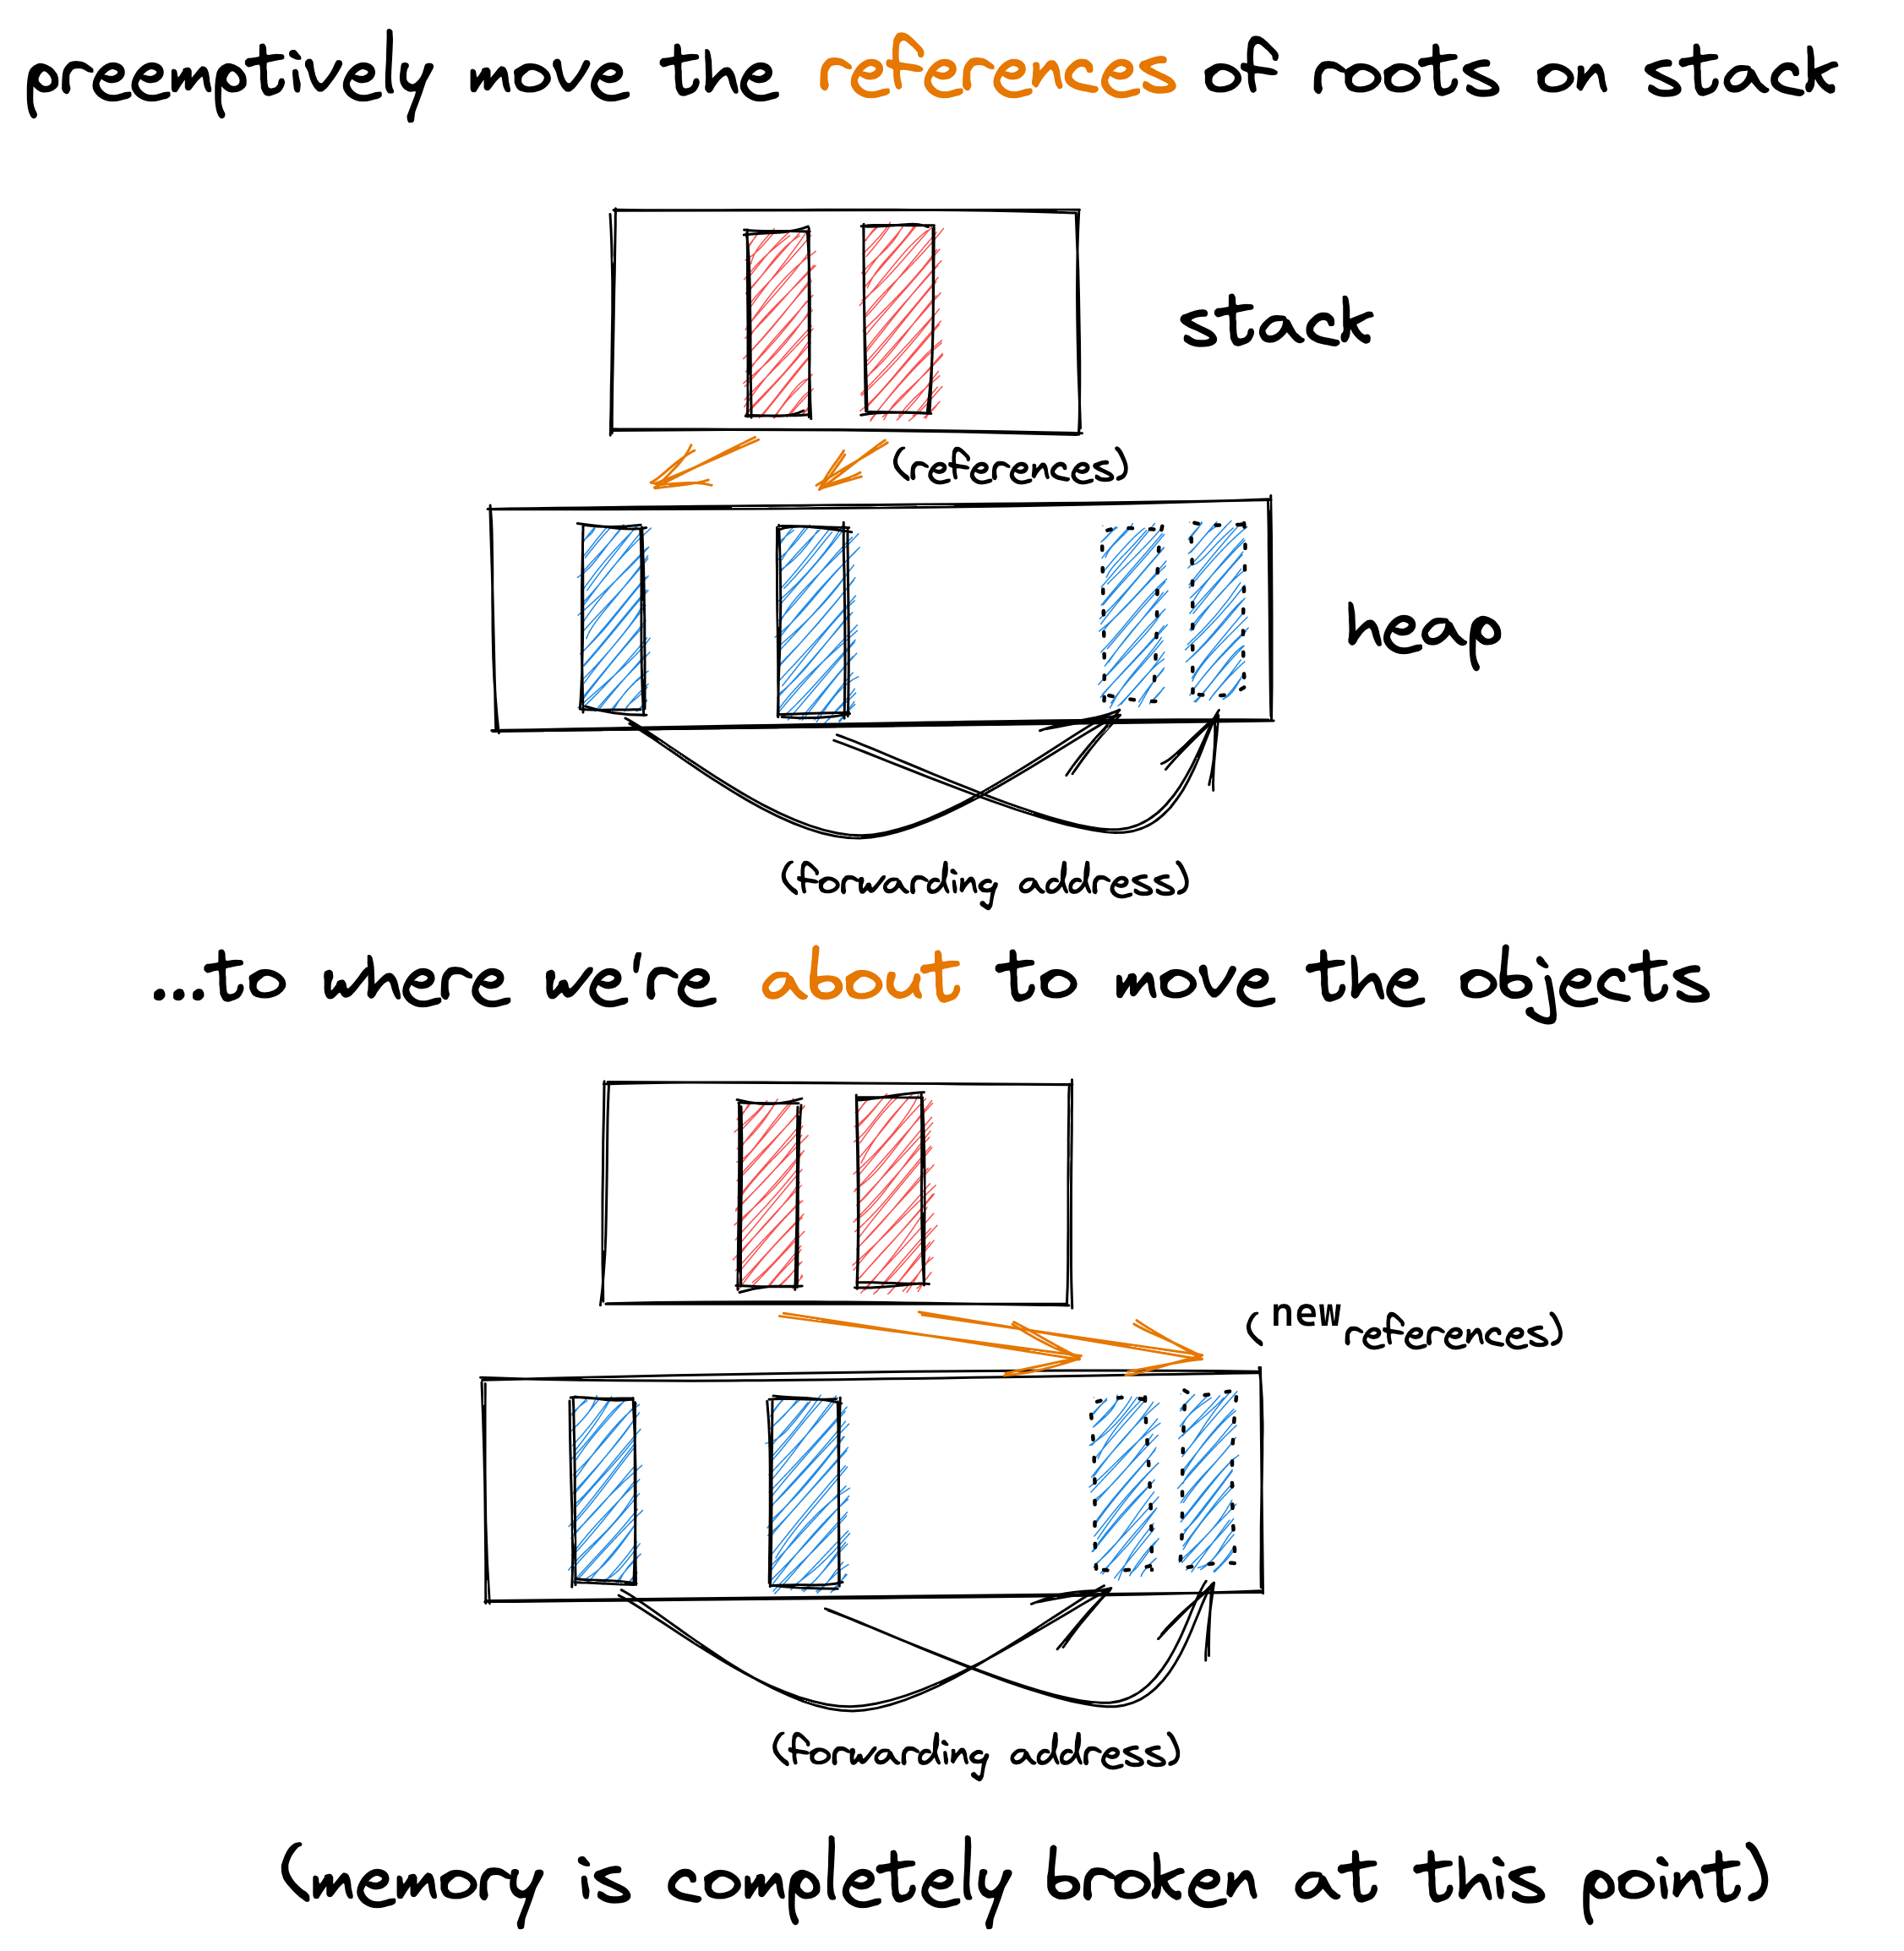
\includegraphics[scale=0.3]{pics/update-references.png}
    \caption{Updating references in the compact step of mark compact, visualized.}
\end{figure}

Finally, we can actually move the objects over to where their \verb+forwarding_address+ points to

\begin{figure}[H]
    \centering
    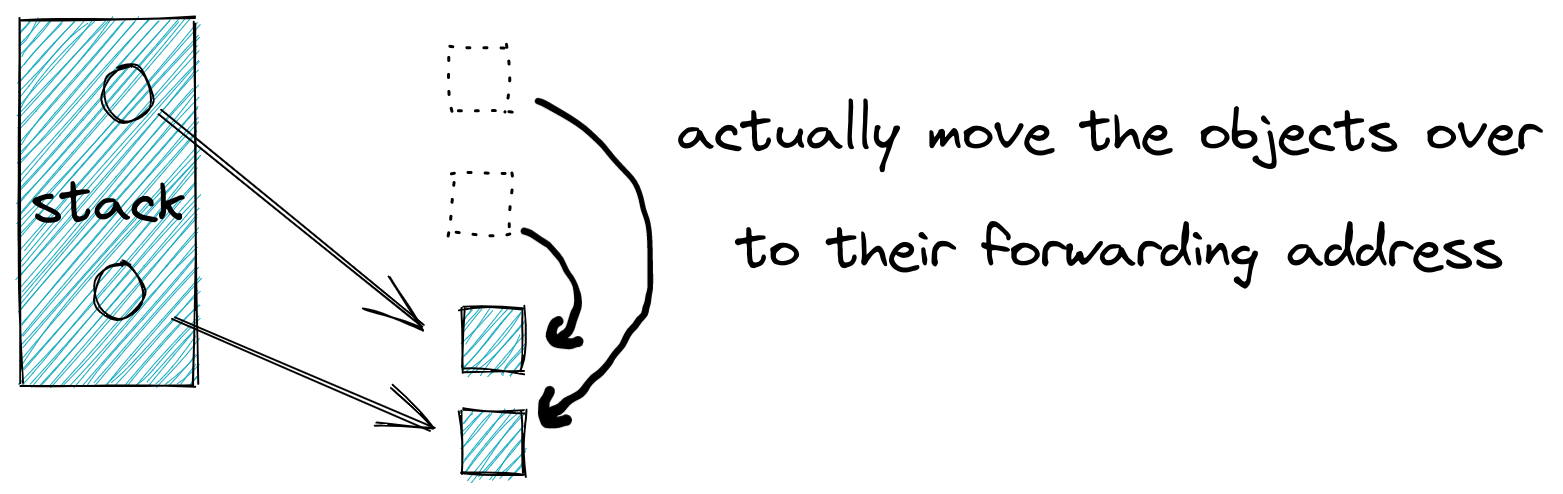
\includegraphics[scale=0.25]{pics/actually-move.png}
    \caption{Actually moving objects, the "compact step" in the compact step of mark compact, visualized.}
\end{figure}

We do this by traversing the heap a 3rd time, then making \mintinline{rust}{std::mem::swap} calls between where the object is currently located and their \verb+forwarding_address+. It's important to note here, that the sliding mark-compaction algorithm maintains the order of which the objects were on in the original heap, as well as moves objects more closely together towards the beginning end of memory, which is why the LISP 2 algorithm is known as a ``sliding'' implmentation of the mark-compact algorithm..

The order is important in the comparison between mark-compact and stop-copy garbage collection algorithms, because Cheney's stop-copy collection algorithm does not preserve the order of objects in memory.

\subsection{Cheney's Stop-and-Copy Algorithm}

The second type of garbage collector investigated in this paper is Cheney's stop-and-copy algorithm, which uses double the memory of the LISP 2 mark-compact algorithm, but in return, is able to mark and copy objects all in one pass.

When initializing the heap using this algorithm, the initial contiguous heap is split into two sections, named a \verb+from_space+ and a \verb+to_space+ \cite[Chapter~2]{gc_handbook}.

\begin{figure}[H]
    \centering
    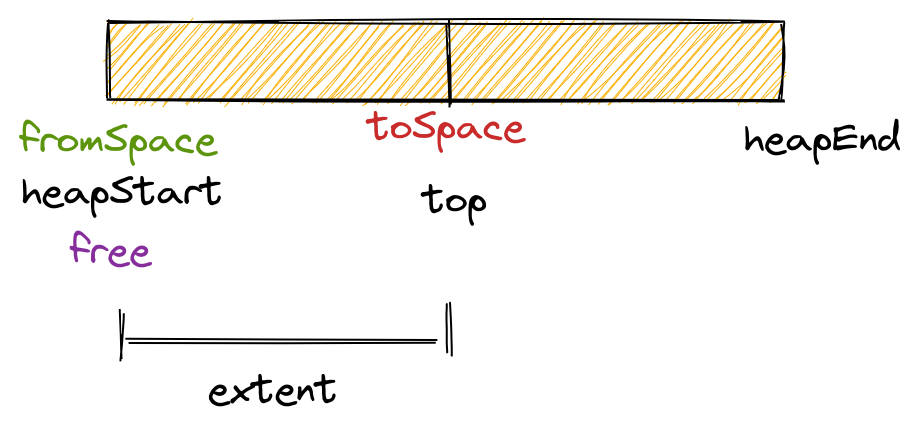
\includegraphics[scale=0.3]{pics/split-heap-diagram.png}
    \caption{Picture of what the heap looks like for a stop-and-copy algorithm}
\end{figure}

Like the mark-compact garbage collector, on every allocation, it checks if the heap has enough free space by attempting to bump the \verb+free+ pointer and check if it's less than the \verb+top+ of the heap.

\begin{figure}[H]
    \centering
    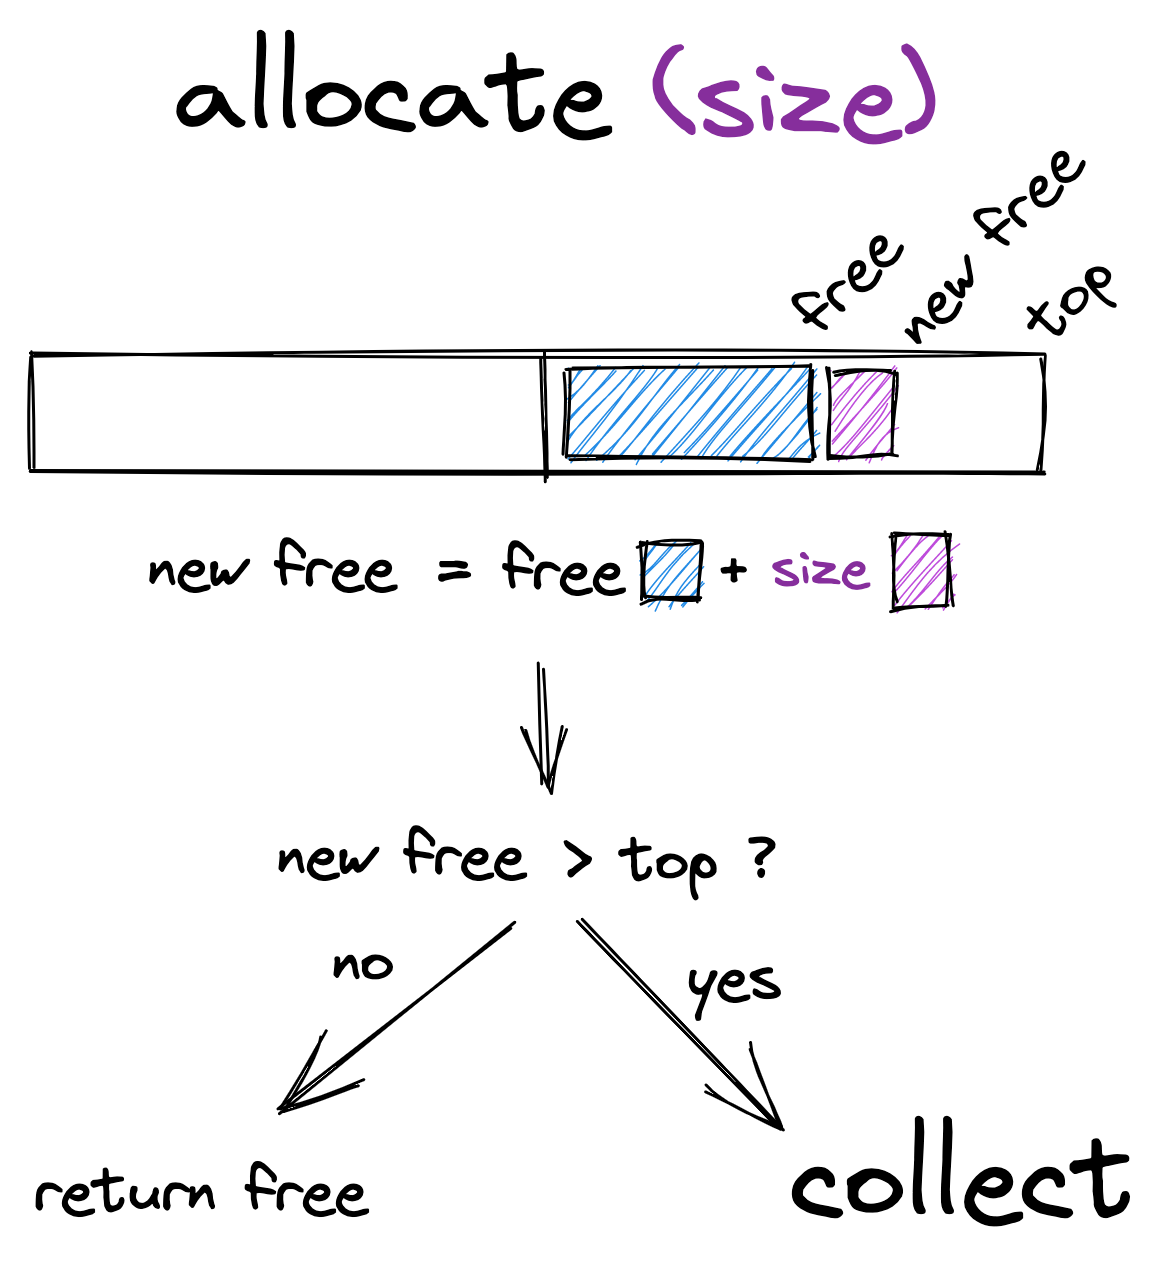
\includegraphics[scale=0.3]{pics/allocation.png}
    \caption{What checking for allocations looks like.}
\end{figure}

\begin{minted}[linenos, breaklines]{rust}
// allocates a new node to the heap
fn alloc(&mut self, node: Node, stack: &mut Stack) -> Result<NodePointer> {
    // check if free is going over fromspace + tospace
    if self.free >= self.top {
        log::trace!("exceeded from space, must run garbage collector");
        // we need to run gc
        self.collect(stack)?;
    }
    if self.free >= self.top {
        return Err("gg collection didn't result in any amount of garbage collected".into());
    }

    // set the node id to where the top of the heap is
    let node_pointer = NodePointer::from(self.free);
    // add it to the heap
    self.committed_memory[usize::from(node_pointer)] = node;
    // bump the free pointer
    self.free += 1;

    Ok(node_pointer)
}
\end{minted}

In this case, because the heap is split in half, we check that the \verb+free+ is not greater than the end of the heap but rather that it is not greater than half of the size of the heap. Once the heap does end up filling up, we can no longer allocate a new object on the heap and thus must call the \verb+collect()+ function of the stop-and-copy garbage collection algorithm.

\subsubsection{Cheney's Algorithm}

Right as we jump into the collect function, we flip the \verb+from_space+ with \verb+to_space+.

\begin{minted}[linenos, breaklines]{rust}
    // first we swap from space with tospace
{
    std::mem::swap(&mut self.from_space, &mut self.to_space);
    // set free to be at the bot of the new to_space
    self.free = self.to_space;
    // set top to be to_space plus the extent
    self.top = self.to_space + self.extent;
}
\end{minted}

\begin{figure}[H]
    \centering
    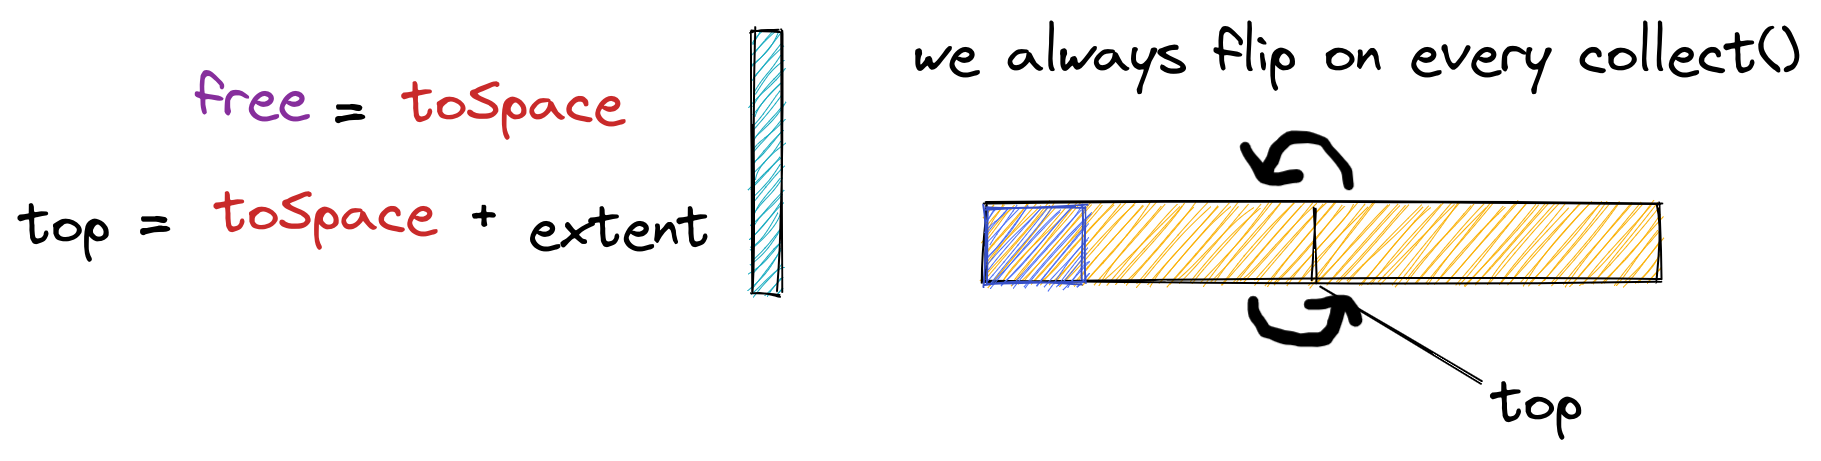
\includegraphics[scale=0.25]{pics/flipping.png}
    \caption{flipping}
\end{figure}

Then we follow that by copying the initial children of the roots reachable by the program into \verb+to_space+. Note that the references that these children newly copied to \verb+to_space+ hold still point to objects in \verb+from_space+

\begin{minted}[linenos, breaklines]{rust}
// next we populate the initial "working list" with roots
{
    // copy the roots over
    // this technically adds them to the worklist
    for root in &mut stack.roots {
        for child in &mut root.children {
            // make sure to update the root refs to point in the right place
            *child = self.copy(*child)?;
        }
    }
}
\end{minted}

Inside the \verb+copy+ function we use above to move the children of the roots over, we update the \verb+forwarding_address+ of their old location on \verb+from_space+ to point to their new location on \verb+to_space+.

\begin{minted}[linenos, breaklines]{rust}
/// copy function
pub fn copy(&mut self, node_pointer: NodePointer) -> Result<NodePointer> {
    // if object has a forwarding address, it means that we've already moved it
    // over to to space, so we can just return its reference
    if let Some(forwarding_address) = self.get(node_pointer).unwrap().forwarding_address {
        Ok(forwarding_address)
    } else {
        // otherwise, like in the mark-compact algorithm, we calculate the
        // location of where this object should exist in to space by bumping the
        // free pointer.
        let new_node_pointer = NodePointer::from(self.free);
        // now we use `.swap()` to move nodepointer current location to its new
        // location free
        self.committed_memory
            .swap(usize::from(node_pointer), usize::from(new_node_pointer));

        // and remember to set the forwarding address of the moved nodepointer
        // to none. This effectively unmarks it in preparation for the next
        // `collect()` cycle, similar to what we do in the mark compact
        // algorithm.
        self.get_mut(new_node_pointer).unwrap().forwarding_address = None;

        // now update the old forwarding address to include itself. This
        // effectively 'marks' the object to make sure that it isn't copied over
        // again. Keep in mind that this object in to space is basically
        // complete garbage except for its forwarding address part
        self.get_mut(node_pointer).unwrap().forwarding_address = Some(new_node_pointer);

        // also remember to bump the free pointer, as we just effectively
        // allocated something to `to_space`
        self.free += 1;

        // finally, we can return the new_node_pointer
        Ok(new_node_pointer)
    }
}
\end{minted}

\begin{figure}[H]
    \centering
    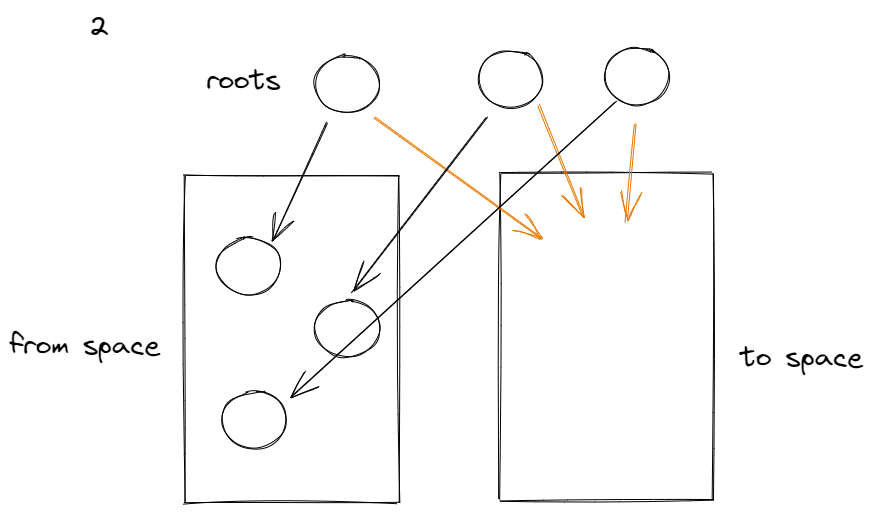
\includegraphics[scale=0.3]{pics/visualization-of-worklist.png}
    \caption{The algorithm for stop and compact. During the collect function, objects in from space are copied to to space, and their forwarding addresses are updated to point to the copied objects in to space.}
\end{figure}

Now, the objects and references of objects in \verb+to_space+ effectively act as a worklist. We repeatedly iterate over the objects in \verb+to_space+, until we reach the end of all the objects in \verb+to_space+. For every object that we then encounter (including the roots that we just moved), we find their references, move them over to \verb+to_space+ if we haven't already, and then update the references to point to \verb+to_space+. (If their references have already been moved, then we can just use their \verb+forwarding_address+ that we updated on the \verb+from_space+ to point to the right location).

\begin{minted}[linenos, breaklines]{rust}
    // now we process all the references of the nodes in the worklist as well
    {
    // you might be wondering...  how do we do `for each node in worklist`?
    // 
    // well, so long as the scan does not catch up to free that is, so as long
    // as we have not processed every single "copied" oject on the heap, keep on
    // going
    while scan < self.free {
        let scan_node_pointer = NodePointer::from(scan);
        // get all references, or children of the object that was recently
        // copied to tospace
        for i in 0..self.get(scan_node_pointer).unwrap().children.len() {
            // set the reference to whatever the forwarding address stored
            // inside the reference is, or copy it
            // 
            // now the reference should now be pointing to copied objects in tospace no matter what
            self.get_mut(scan_node_pointer).unwrap().children[i] =
                self.copy(self.get(scan_node_pointer).unwrap().children[i])?;
            // the references get added to the worklist automatically
        }
        // don't forget to bump the scan pointer
        scan += 1;
    }
}
\end{minted}

Upon reaching the end of the \verb+to_space+, garbage collection is done, because all live objects have been copied to the the effective heap. At this point, the \verb+from_space+ is basically ignored, and the \verb+to_space+ becomes the effective heap, until the next cycle of garbage collection occurs.


\section{Experiment}

From the algorithms above, one can infer that for a garbage collector, there are two areas where pure performance can be measured. This is during the \verb+collect()+ part of the algorithm, when the graph of live objects is being traversed and objects are being moved to their compacted points, as well as the runtime performance of the program, when the objects on the heap are being accessed.

To measure the collection performance, garbage will be generated in a graph of objects. And to measure the runtime performance, the graph of all objects will be traversed, and the values that each of the objects will be summed up.

To generate the testing data, the custom abstraction of a garbage collected data structure will be used \cite{youtube_introductory_video}. A dead simple binary tree will be filled with a predetermined number of \(1,000,000\) objects. Every node is first pushed to the end of the free space on the vector, and children are added as indices, which are an abstraction of pointers. Each node will have two children until the leaf nodes of the tree are reached.

Then, a seeded random number generator will be used to link \(500,000\) random objects from the first half of the tree to \(500,000\) random objects in the latter half of the tree (via adding their indices as children).

Finally, a number of children will be removed from a range of parents in the tree, which will generate garbage: there will be two sets of data, one with a large number of live objects remaining after the garbage collection, and one with a smaller number of live objects remaining (the number of removed nodes will be shown in the data below).

The testing framework used in this will be the \verb+criterion+ crate in Rust, which automatically runs each function for a set amount of time in the beginning to ``normalize'' the caches, which is especially important \cite{a_unified_theory_of_garbage_collection} for the comparison of garbage collection algorithms, as the way objects are arranged in memory will affect the layout of objects in the cache, which is important to keep consistent. It also determines the number of tests to run and takes the average of all of them, the information of which will be presented in the data below.

\section{Conclusion}
\subsection{Areas of Error}

Though, it should be noted that the data structure used to represent the objects, the way the objects were linked, and the values that the objects held are all very specific things that could lead to a couple biases for one algorithm or another based off these things alone.

A tree with links here and there is one type of data structure.

Another shortcoming is that heaps are acted on for a long period of time. Especially for the stop-and-copy algorithm: in the first iteration it's runtime performance was almost just as good as mark-compact and it had a \verb+collect()+ speed that was twice as fast.

Another thing was the fact that the "marking bitmap" the mark-compact algorithm algorithm used required regeneration everytime garbage needed to be collected. No universal implementation of the marking bitmap was found for the LISP-2 style mark compact algorithm. The specific implmentation in this paper chose to use the builtin langauge quicksort 3 algorithm to order the indices after marking. This could've introduced a confounding variable, since if sorting algorithms were used with a higher time complexity the stop-and-copy algorithm would've been observed to be faster.

\subsubsection{Side note on page}

In most modern computers, including Windows and Linux, memory in a program is virtual memory, and each range of virtual memory maps to a range of physical memory addresses on hardware \cite{code_project}. These are stored in tables, and there is a \verb+page+ storage allocated for each address in order to link these virtual addresses to physical addresses. However, looking up these values is actually fairly expensive in terms of performance, so physical hardware has a lookup cache, with around the last 500 pages stored in it. Therefore, when objects are closer together in memory or when the order is maintained, it might provide a locality bonus, therefore increasing performance. However, it is still important to note that this implementation still traverses the heap itself 3 times in order to compact objects, which would be a fairly expensive thing to do on large heaps.

However, despite the fact that Cheney's stop-and-copy algorithm has much fewer steps than the mark-compact garbage collector, it has several downsides. Apart from the most obvious thing being the heap split in half, it's important to note that the way the worklist is traversed in this algorithm, it's effectively breadth-first by reference. Therefore, when objects are moved, their original order is not preserved, unlike with the mark-compact garbage collector. This could negatively affect program performance, because parents have the possibility of being separated from their children, resulting in large differences in locality despite the heap being compacted.

It should be noted that mark-and-compact and stop-and-copy garbage collectors are also both moving garbage collectors, meaning that memory is swapped and copied around throughout the garbage collection cycle. Moving large surviving objects multiple times will inevitably lead to poor performance \cite[Chapter~4]{gc_handbook}.

Stop-and-copy garbage collection actually moves more than mark-compact garbage collection, because there isn't the possibility of objects staying in place and already being compacted. But on the flipside, instead of having to traverse the heap 3 times to achieve heap compaction, the heap is effectively only traversed one time in one fell swoop.

And while mark-and-copy garbage collection is using double the memory that mark-compact is, it is still very elegant how a worklist or queue is not needed to  get through marking, and neither is a marking bitmap. By traversing the heap 3 times less, one might infer that for large heaps, the semi-space algorithm would outperform the mark-compact garbage collector algorithm.

% What is the mutator again?
% Revise images
% What is the l2 cache?
% ~50 mb cache on the CPU responsible for quickly accessing data, is orders of magnitude faster than RAM or harddrive?
% When does it get proced when...
% Bugs: https://github.com/SpicyRicecaker/gc-representation-rs

\section{Works Cited}

\printbibliography

\end{document}